\newpage
\begin{center}
	\textbf{\large ГЛАВА 4 \\ МОДЕЛИРОВАНИЕ И СБОРКА}
\end{center}
\refstepcounter{chapter}


% \section*{}
\addcontentsline{toc}{chapter}{ГЛАВА 4}
\section{Общие требования к физической модели четырехногого робота}\label{C4_1}

Все четвероногие животные при движении сохраняют равновесие почти исключительно за счет динамической устойчивости. Изначально план чередования опорных и свободных положений ног заключался в переключении фаз по принципу ноги 1-4 опорная фаза, ноги 2-3 свободная, как показано на рисунке \ref{cycle_wanted}. Зелеными стрелками обозначены фазы свободного положения, а красными опорного. Однако, такой подход не совсем точен, хоть и вполне логичен.
\begin{figure}[h!]
	\begin{center}
		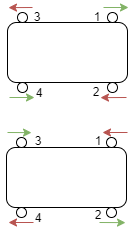
\includegraphics[width=0.3\textwidth]{cycle_wanted}
		\caption{Смена опорных и свободных фаз.}
		\label{cycle_wanted}
	\end{center}
\end{figure}

  В случае искусственных шагающих аппаратов походка должны быть определена таким образом, чтобы центр тяжести аппарата постоянно находился внутри треугольника, вершинами которого являются конечности, находящиеся на данный момент времени в опорном положении (рисунок \ref{diagrama}). На практике эта возможность была реализована д-ром Такути из Научно-исследовательского центра проблем механики. Под его руководством был разработан шагающий аппарат с четырьмя конечностями, у которых скорость движения в фазе восстановления подобрана так, что длительность этой фазы втрое меньше длительности каждой рабочей фазы. В результате в данный момент времени лишь одна нога робота находится в воздухе, а корпус опирается на три остальные, сохраняя тем самым статическую устойчивость. 
  
  Показанные на рисунке заштрихованные треугольники (так называемые опорные треугольники) образованы вершинами, которые соответствуют текущим точкам касания опорной поверхности какими-либо тремя из четырех ног робота. Например, в состоянии, соответствующем рисунку \ref{diagrama}, опоры касаются три ноги - А, В, С, а четвертая нога - D, будучи в фазе восстановления, находится в воздухе. Для обеспечения статической устойчивости принципиально важное значение имеет правильный выбор порядка чередования (сдвиг фаз) четырех ног в процессе движения аппарата. В момент времени, отраженный на диаграмме 1, нога В только что коснулась земли и сейчас занимает опорное положение, нога А также касается земли, но находится уже во второй половине своей рабочей фазы, а нога С - еще в первой половине собственной рабочей фазы. Нога D, находящаяся в момент наблюдения в воздухе, быстро заканчивает фазу восстановления, и к моменту времени, которому соответствует диаграмма 2, она уже опускается на землю, переходя в опорное положение. К этому моменту нога А завершила свою рабочую фазу и, оторвавшись от земли, переходит в фазу восстановления; нога В находится в первой половине, а нога С - во второй половине своих рабочих фаз. Аналогично в следующие моменты времени, которым соответствуют диаграммы 3 и 4, в фазу восстановления переходят друг за другом нога С и нога В. 
  
  При таком порядке чередования ног в любой момент времени, когда одна из ног робота находится в фазе восстановления, центр тяжести аппарата обязательно будет лежать внутри треугольника, образованного тремя ногами, находящимися не в рабочей фазе (опирающимися на землю).
  
\begin{figure}[h!]
  	\begin{center}
  		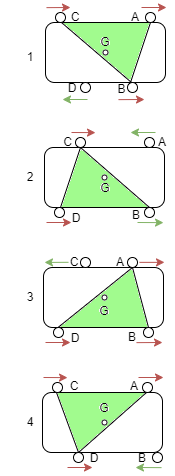
\includegraphics[width=0.3\textwidth]{diagrama}
  		\caption{Смена опорных и свободных фаз с учетом тяжести}
  		\label{diagrama}
  	\end{center}
\end{figure}

\newpage

\section{Проектирование ног}\label{C4_2}

В разделе \ref{C1_2} были представлены особенности конструкции и основные проблемы, которые необходимо решить перед производством деталей. 

Для минимизации проблем, связанных с соосностью отверстий, отношениями и масштабами между конструкциями перед этапом печати, были использовали трехмерные твердотельные чертежи при проектировании ног в формате 3D (рисунок \ref{leg_3D}). В качестве материала для изготовления деталей ног был выбран пластик, который используется при печати с помощью 3D-принтера, поскольку уникальная конструкция ног не позволяет использовать доступные металлические изделия для сборки. Кроме того, использование пластика значительно снижает вес конструкции, что позволяет использовать менее мощные двигатели для создания прототипа. Напечатанные и собранные конструкции ног отображены на рисунках \ref{leg2}, \ref{leg3}.  
\begin{figure}[h!]
	\begin{center}
		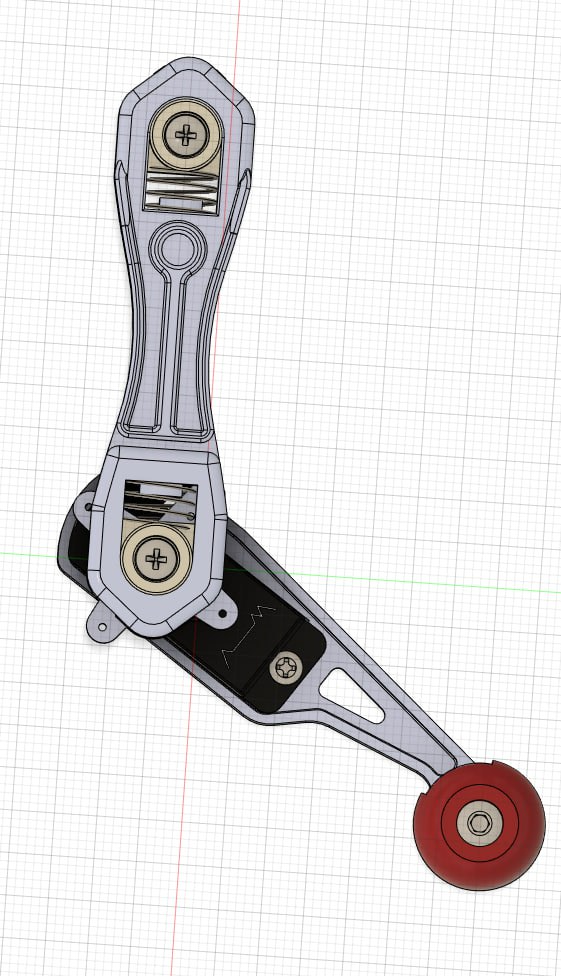
\includegraphics[width=0.45\textwidth]{leg_3D}
		\caption{Твердотельный чертеж ноги робота}
		\label{leg_3D}
	\end{center}
\end{figure}

\newpage
Сервоприводы, как в сочленении ног, так и в месте соединения с корпусом, закреплены к ползуну, который в свою очередь подпирается пружиной. Ползун обладает "Т" \space образной формой (рисунок \ref{polzun}), которая поддерживает его в плоскости ноги и не дает покинуть область конструкции. 

Пружина служит в качестве демпфера, который гасит ударные воздействия на вал двигателя при движении робота, а также оказывает некоторое полезное сопротивление при резком изменении угла поворота двигателя, что не раз спасало прототип при "живом" \space тестировании походки.

\begin{figure}[h!]
	\begin{center}
		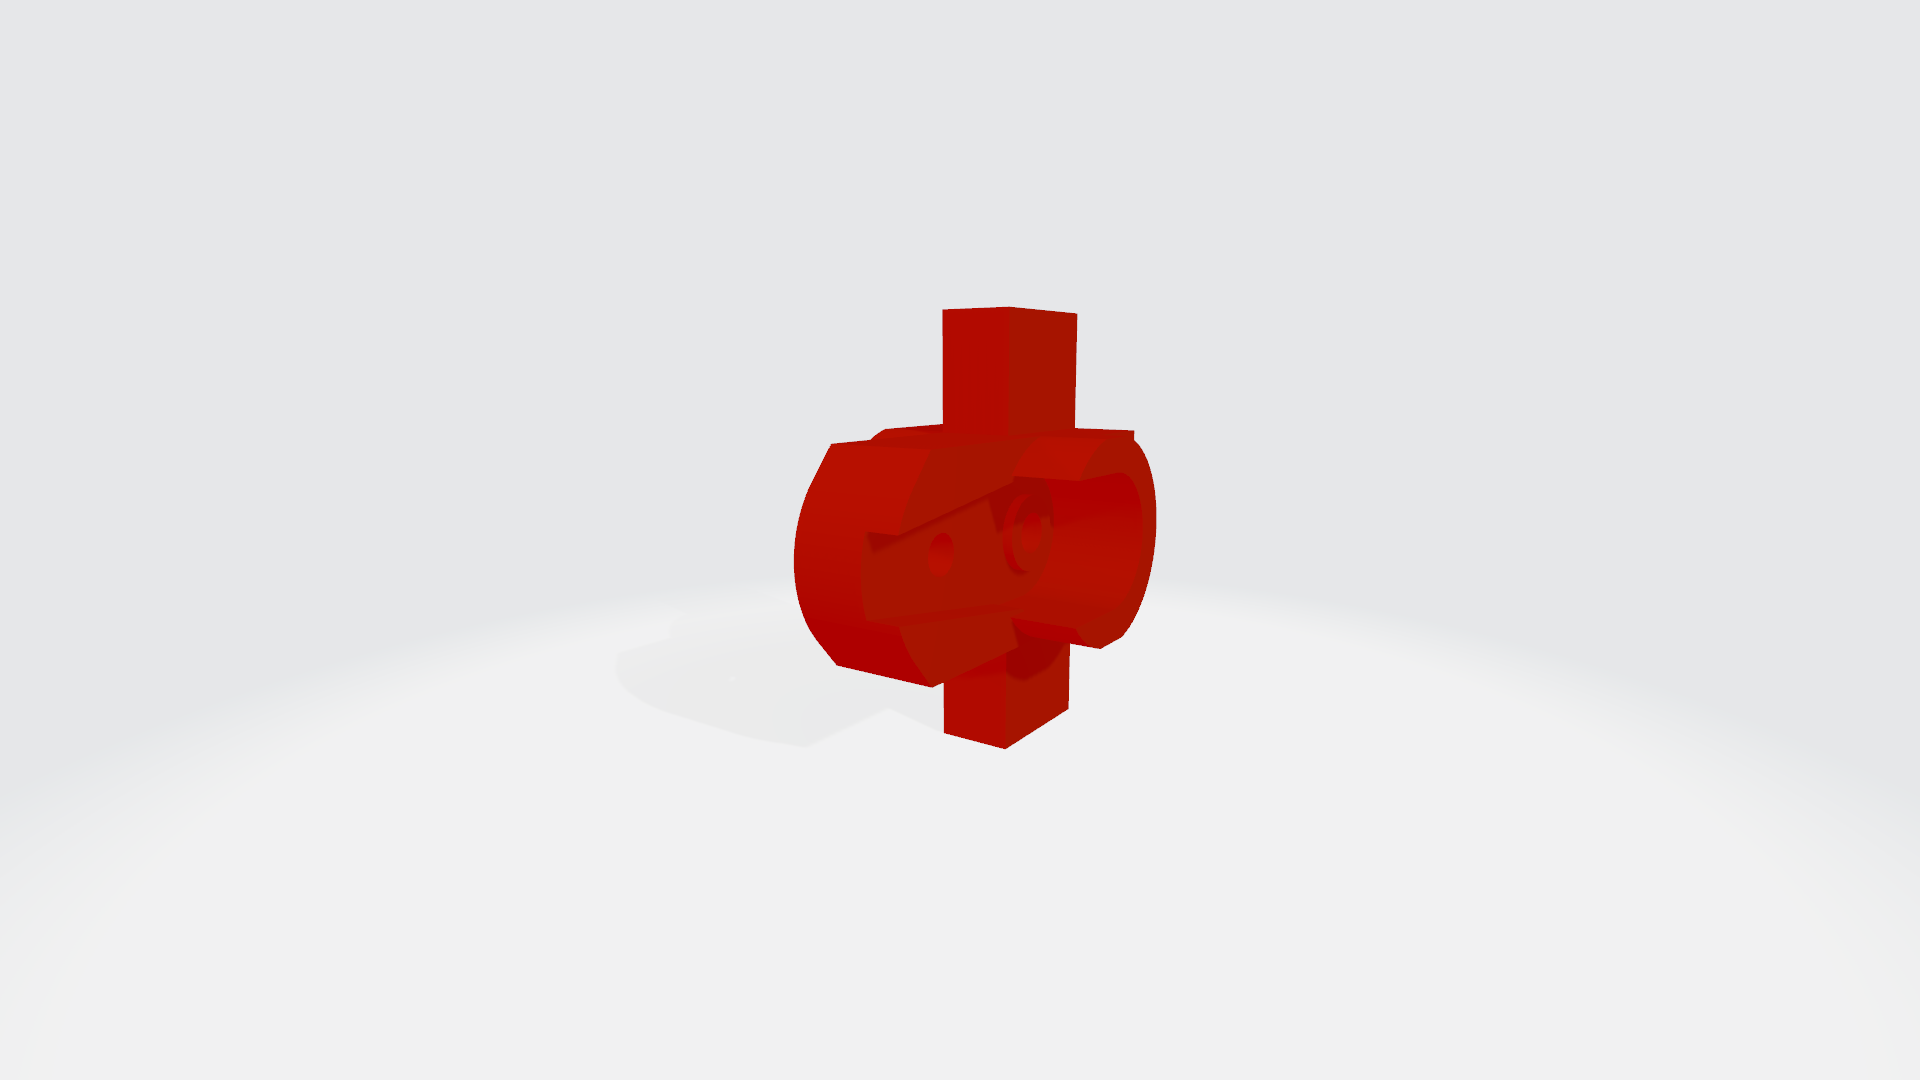
\includegraphics[width=0.8\textwidth]{polzun}
		\caption{\text{''T''} - образный ползун}
		\label{polzun}
	\end{center}
\end{figure}
\newpage
\begin{figure}[h!]
	\begin{center}
		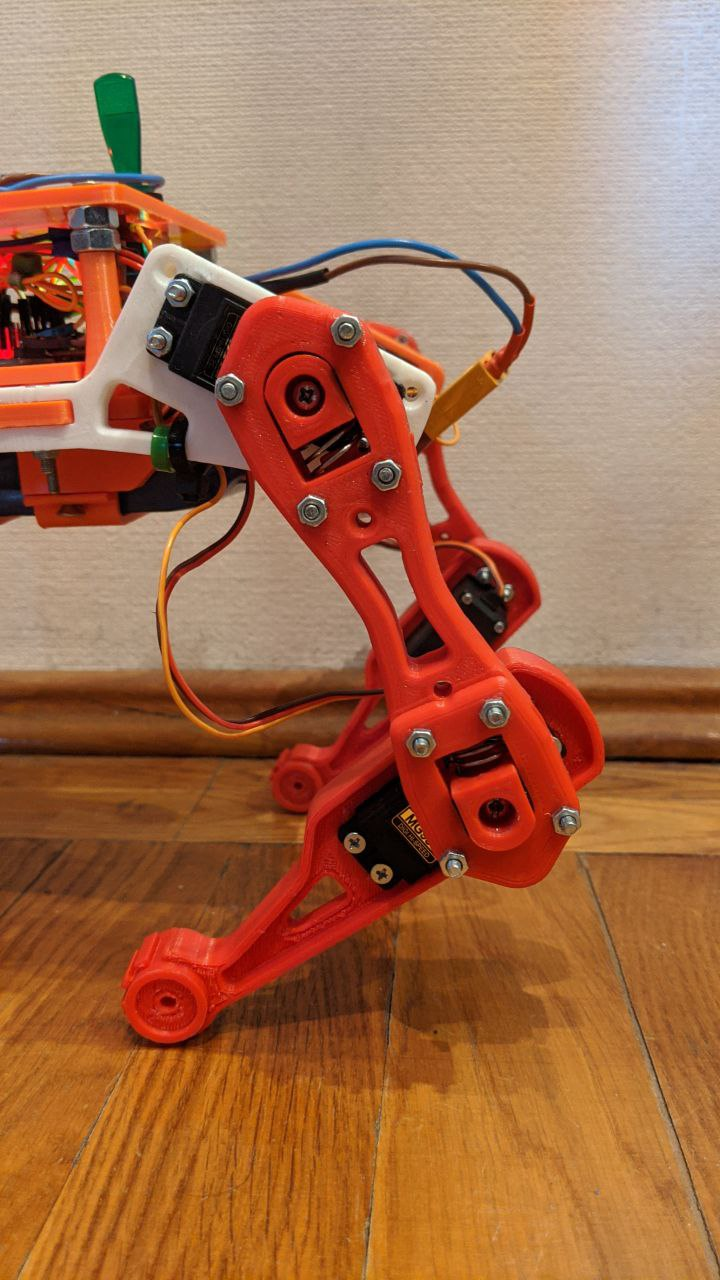
\includegraphics[width=0.4\textwidth]{leg2}
		\caption{Напечатанная нога в сборке}
		\label{leg2}
	\end{center}
\end{figure}

\begin{figure}[h!]
	\begin{center}
		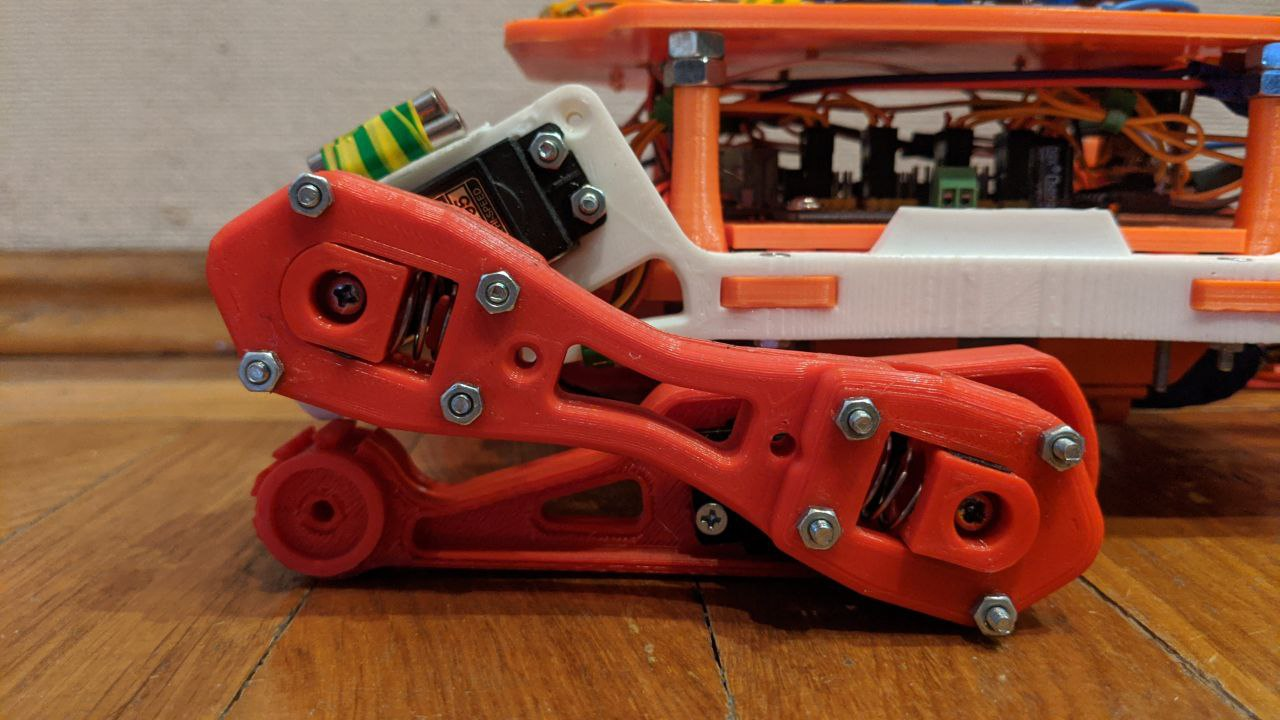
\includegraphics[width=0.5\textwidth]{leg3}
		\caption{Робот в исходном положении до инициализации}
		\label{leg3}
	\end{center}
\end{figure}

\newpage
\section{Проектирование корпуса}\label{C4_3}

Корпус для робота представляет из себя поперечные пластины (рисунок \ref{plastina}), соединенные с лонжеронами. Данные пластины несут функцию размещения электронных компонентов и создания жесткости конструкции. 

\begin{figure}[h!]
	\begin{center}
		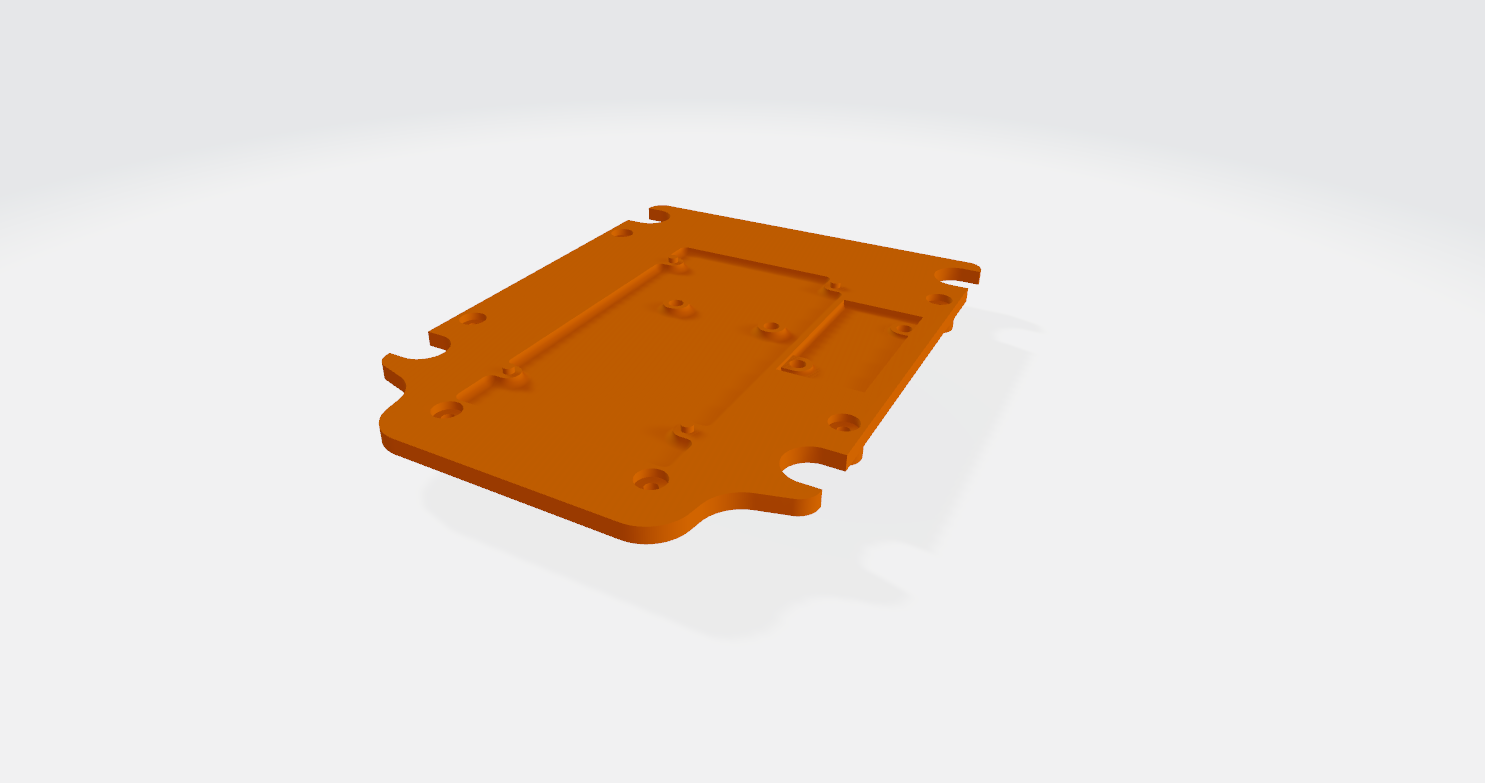
\includegraphics[width=0.8\textwidth]{plastina}
		\caption{Твердотельный чертеж пластины корпуса}
		\label{plastina}
	\end{center}
\end{figure}

В качестве детали к которой крепятся ноги робота, были выбраны лонжероны, также изготовленные из пластика (рисунок \ref{longeron}). Данное решение было принято из-за легкости материала и достаточной жесткости, необходимой для удержания закрепленных деталей. 

\begin{figure}[h!]
	\begin{center}
		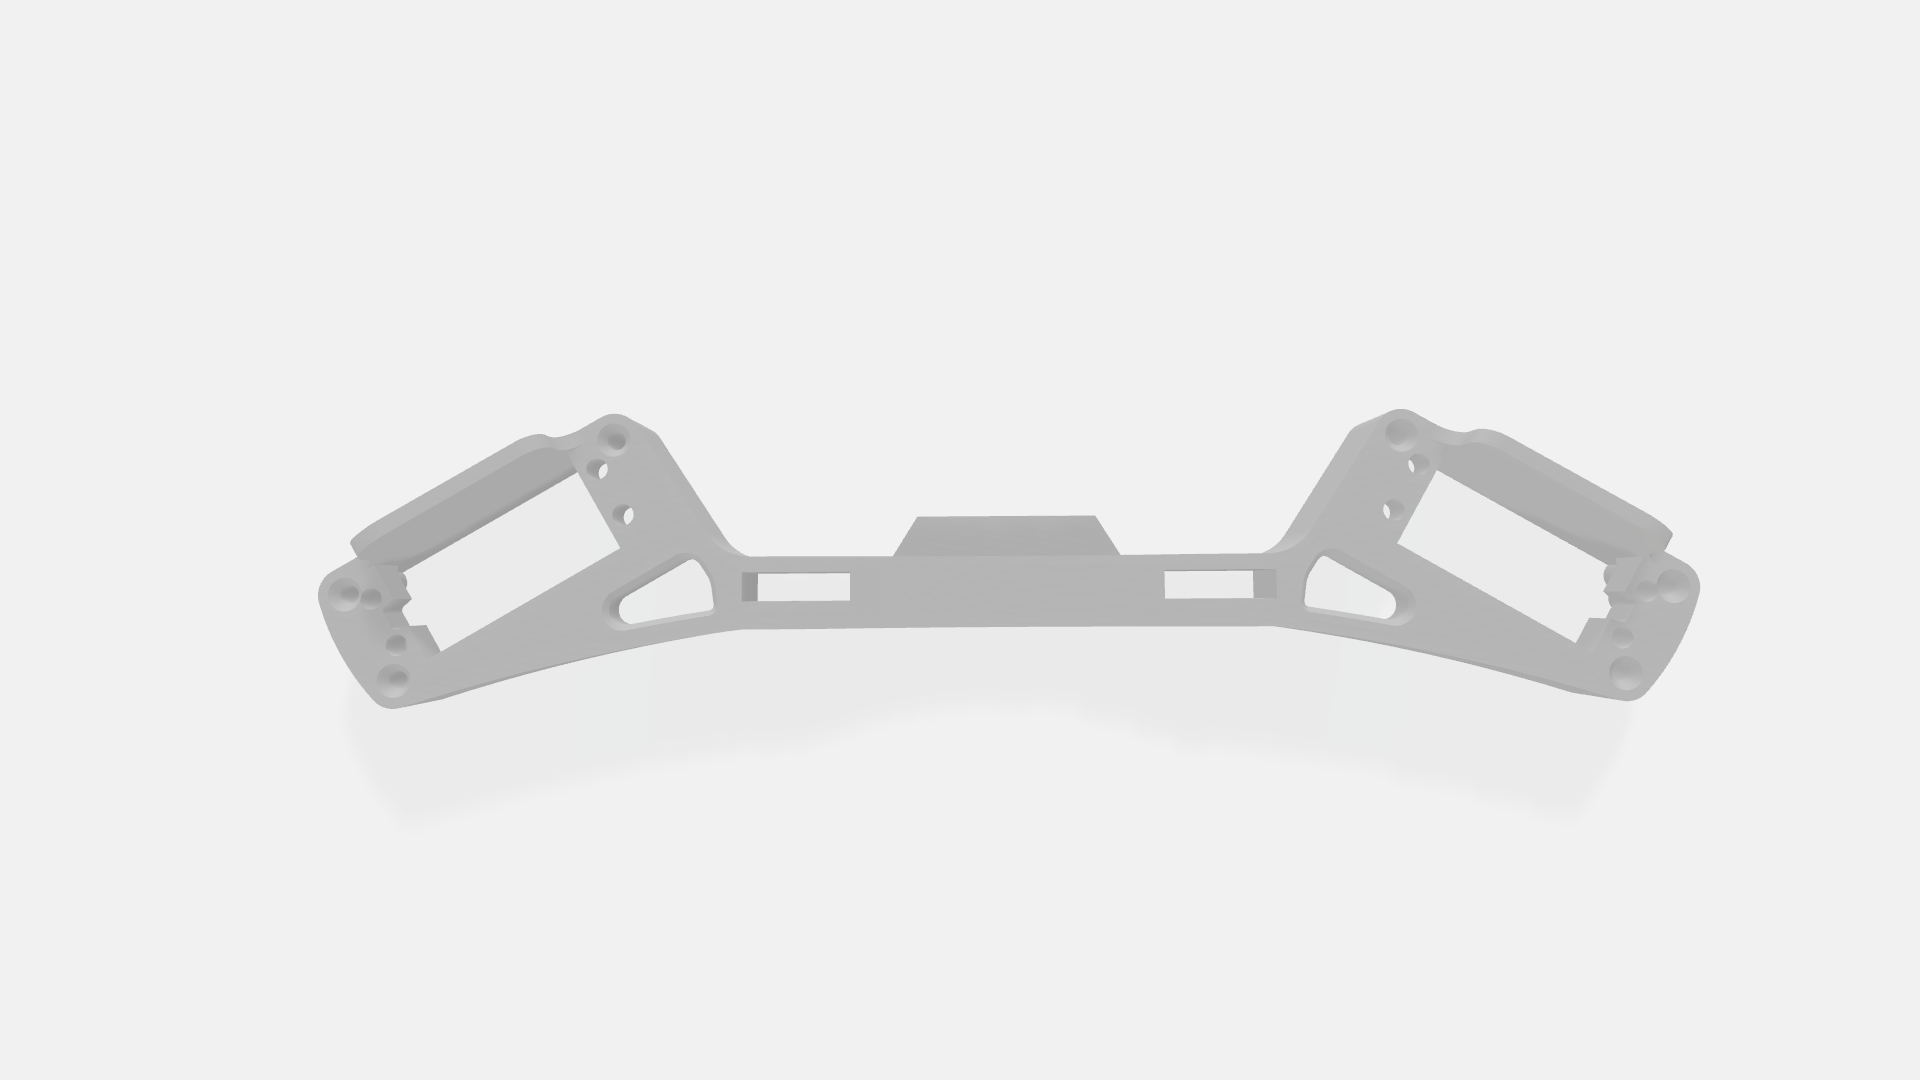
\includegraphics[width=0.8\textwidth]{longeron}
		\caption{Твердотельный чертеж лонжерона корпуса}
		\label{longeron}
	\end{center}
\end{figure}
\pagebreak
В отличие от ног, к корпусу были только минимальные требования, а именно небольшой вес и удобное расположение модулей для последующего подключения. На верхнем уровне корпуса расположены DC/DC преобразователи и трехосевой гироскоп акселерометр MPU6050. На нижнем уровне располагается миникомпьютер OrangePi 3 LTS и ШИМ контроллер PCA9685, в то время как с обратной стороны пластины закреплен источник питания в виде Li-Po аккумулятора (более подробно о подборе комплектующих в разделе 4.4).


\section{Выбор комплектующих}\label{C4_4}
	\subsection{Выбор сервоприводов}\label{C4_4_1}
	
Сервопривод - это механический привод, который содержит датчик (для измерения положения, скорости, усилия и других параметров) и блок управления приводом (который может быть электронной схемой или механической системой тяг), что позволяет автоматически поддерживать необходимые параметры на датчике в соответствии с заданным внешним значением (например, положение ручки управления или численное значение от других систем). Сервопривод можно рассматривать как автоматического точного исполнителя, который получает на вход значение управляющего параметра в режиме реального времени и используя показания датчика, стремится создать и поддерживать это значение на выходе исполнительного элемента. 

В данной работе предлагается рассчитать максимальный крутящий момент при худшем случае конфигурации робота. При выборе сервопривода данный параметр особенно значим, так как все остальные характеристики вроде габаритов и мест размещения крепежей у этих типов двигателей мало отличаются. Для того чтобы рассчитать худший случай нагрузки и выбрать подходящий сервопривод, необходимо знать следующие параметры:
\begin{itemize}
	\item Общий вес робота;
	\item Длины ног.
\end{itemize}

Худшей конфигурацией является случай, когда все ноги робота вытянуты в "струнку" (рисунок \ref{badass}). В таком случае серводвигателям необходимо приложить максимальный крутящий момент для возврата в рабочую конфигурацию.

\begin{figure}[h!]
	\begin{center}
		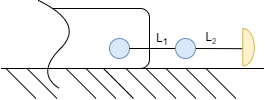
\includegraphics[width=0.5\textwidth]{badass}
		\caption{{Худшая конфигурация для статического случая}}
		\label{badass}
	\end{center}
\end{figure}

Учитывая параметры из таблицы \ref{tablParam}, а также взвесив корпус, с заранее установленными комплектующими, вес робота составляет 1.6 кг. Будем считать, что движения ног для возвращения в исходную конфигурацию будет происходить синхронно, то есть общую нагрузку можно разделить на четыре ноги, что составляет 0.4 кг на одну ногу. Предлагается следующая формула для вычисления максимального момента на одну ногу в случае худшей конфигурации:
 \begin{equation}
	\begin{array}{l}
		M^{\text{крут}}_{\text{макс}} = \frac{m_{\text{роб}}g}{4}(l_{1}+l_{2}),
	\end{array}
	\label{max_moment}
\end{equation}

Исходя из формулы \ref{max_moment} был получен крутящий момент равный 0.8 Нм. В настоящей работе выбрана модель сервопривода MG995, которая полностью удовлетворяет требованиям. Основные характеристики данного привода сведены в таблице \ref{servoParam}.


\begin{table}[h]
	\begin{center}
		\caption{Характеристики сервопривода MG995}
		\label{servoParam}
		\begin{tabular}{| l | l |}
			\hline
			Общий вес   &    55 г \\ \hline
			Размеры (ШхВхГ) & 54х47.2х20 мм\\ \hline
			Крутящий момент & 8.5кгс/см (4.8В), 10кгс/см (6В) \\ \hline
			Рабочая скорость & 0.2с/60$^{\circ}$ (4.8В), 0.16с/60$^{\circ}$ (6В) \\ \hline
			Рабочее напряжение & 4.8В - 7.2В \\ \hline
			Рабочая температура & 0 C$^{\circ}$  - 55 C$^{\circ}$ \\ \hline
			Зона нечувствительности ШИМ & 5мкс \\ \hline
		\end{tabular}
	\end{center}
\end{table} 

Одним из самых главных минусов при работе с сервоприводами является гибкость управления валом двигателя. Резкие изменения угла в серводвигателях являются следствием специфики их конструкции, а если быть точнее, то данная проблема связана с принципом работы потенциометра, который выполняет роль энкодера внутри двигателя. Таким образом принцип регулирования угла поворота состоит в подаче ШИМ сигнала посредством написанного программного обеспечения, сам сигнал преобразуется в напряжение благодаря работе потенциометра и приводит вал в заданное положение с максимальной скоростью. Из этого можно сделать вывод, что в используемых  сервоприводах не имеется обратной связи, и при использовании с тяжелыми объектами будут создаваться лишние нагрузки, которые будут приводить к потреблению тока, особенно это важно по отношению к стартовым токам. В нашем случае такое поведение потенциально приведет к уничтожению редуктора внутри двигателя (рисунок \ref{servo_scheme}), так как движимые объекты инерционные и такое управление для них неприемлемо. Решение этой проблемы подробной разобрано в главе \ref{C5_1}. 

\begin{figure}[h!]
	\begin{center}
		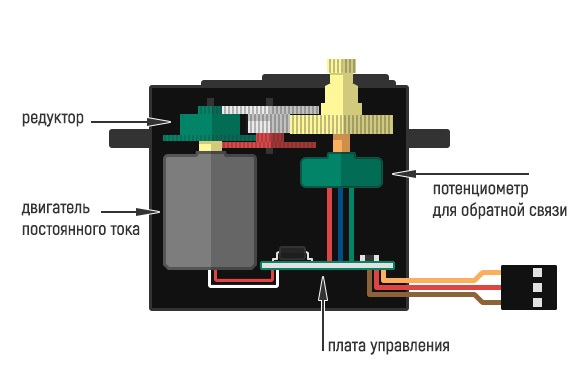
\includegraphics[width=0.7\textwidth]{servo_scheme}
		\caption{Схема сервопривода}
		\label{servo_scheme}
	\end{center}
\end{figure}

Еще одним последствием такого принципа работы выступает осложнение корректной сборки, так как для правильной конфигурации ноги на прототипе сервоприводам требуется калибровка. Иначе говоря, необходимо выставлять крайние положения ног и рассчитывать диапазон ШИМ сигнала и принимаемого угла, чтобы как можно точнее задавать положение ноги в будущем. Это достаточно неприятное следствие, так как каждая единица серводвигателя уникальна и требует отдельной калибровки. Методы калибровки в данной работе разбираться не будут.

\subsection{Выбор управляющей электроники}\label{C4_4_2}
	
В качестве управляющей платы миникомпьютера была выбрана OrangePi 3 LTS (рисунок \ref{orange_pi}). Данный миникомпьютер покрывает все технические требования прототипа сверх нормы, что позволяет не задумываться о методах опрашивания датчиков или скорости обработки информации. Также весомым преимуществом такого компьютера является автономность и наличие встроенной ОС Linux. Такие особенности позволяют использовать плату в привычном для разработчика режиме и не терять время на настройку программного окружения. 	
\begin{figure}[h!]
	\begin{center}
		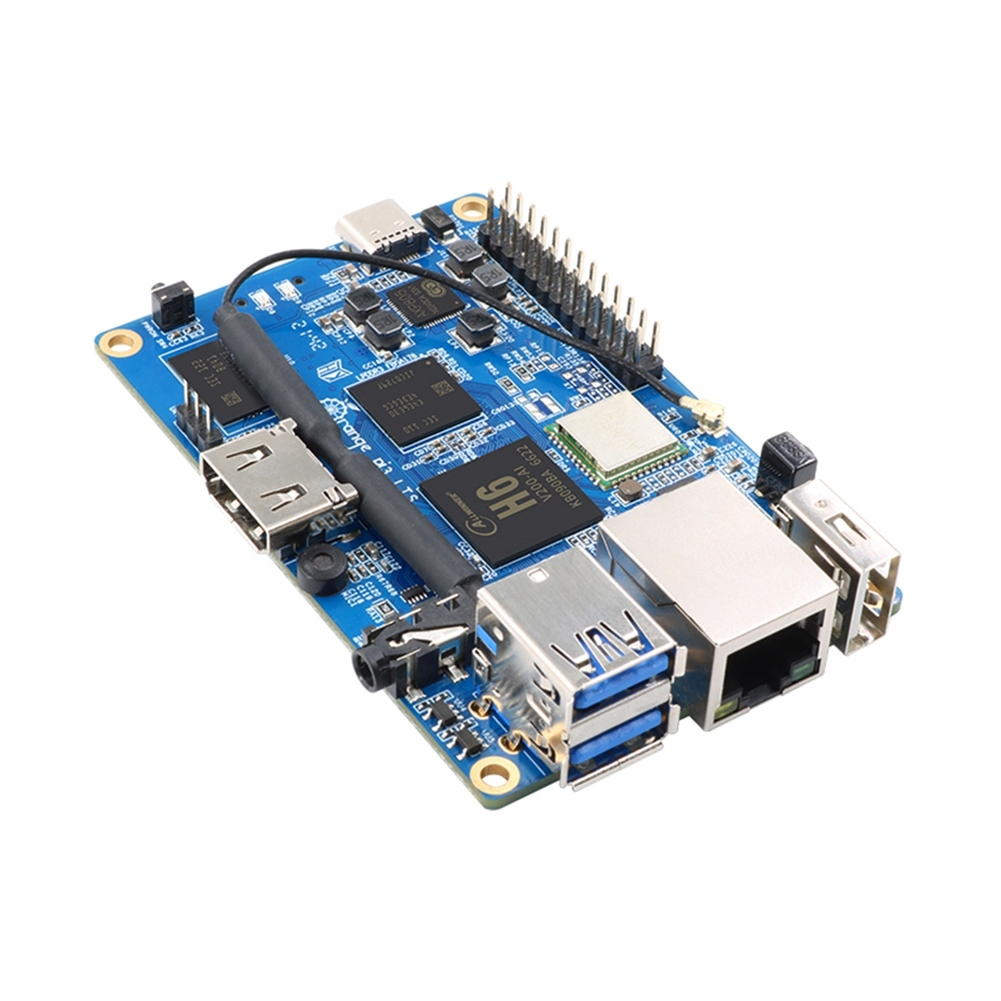
\includegraphics[width=0.4\textwidth]{orange_pi}
		\caption{OrangePi 3 LTS}
		\label{orange_pi}
	\end{center}
\end{figure}

\newpage
Так как OrangePi не поддерживает управление восемью серводвигателями одновременно, было предложено использовать ШИМ контроллер. В качестве данного контроллера был выбран модуль PCA9685. PCA9685 - это высокопроизводительный драйвер сервоприводов, разработанный фирмой NXP Semiconductors. Он обладает шестнадцатью независимыми каналами широтно-импульсной модуляции (PWM), каждый из которых может управлять сервоприводом. Также PCA9685 имеет встроенную функцию автоматического обновления адресов, что позволяет подключать несколько драйверов к одной шине I2C. Такой подход позволяет назначить уникальный адрес для каждого подключения, чтобы добиться одновременного управления большим количеством сервоприводов. Драйвер также поддерживает частоту ШИМ до 1 кГц, что обеспечивает высокую точность управления сервоприводами.

\begin{figure}[h!]
	\begin{center}
		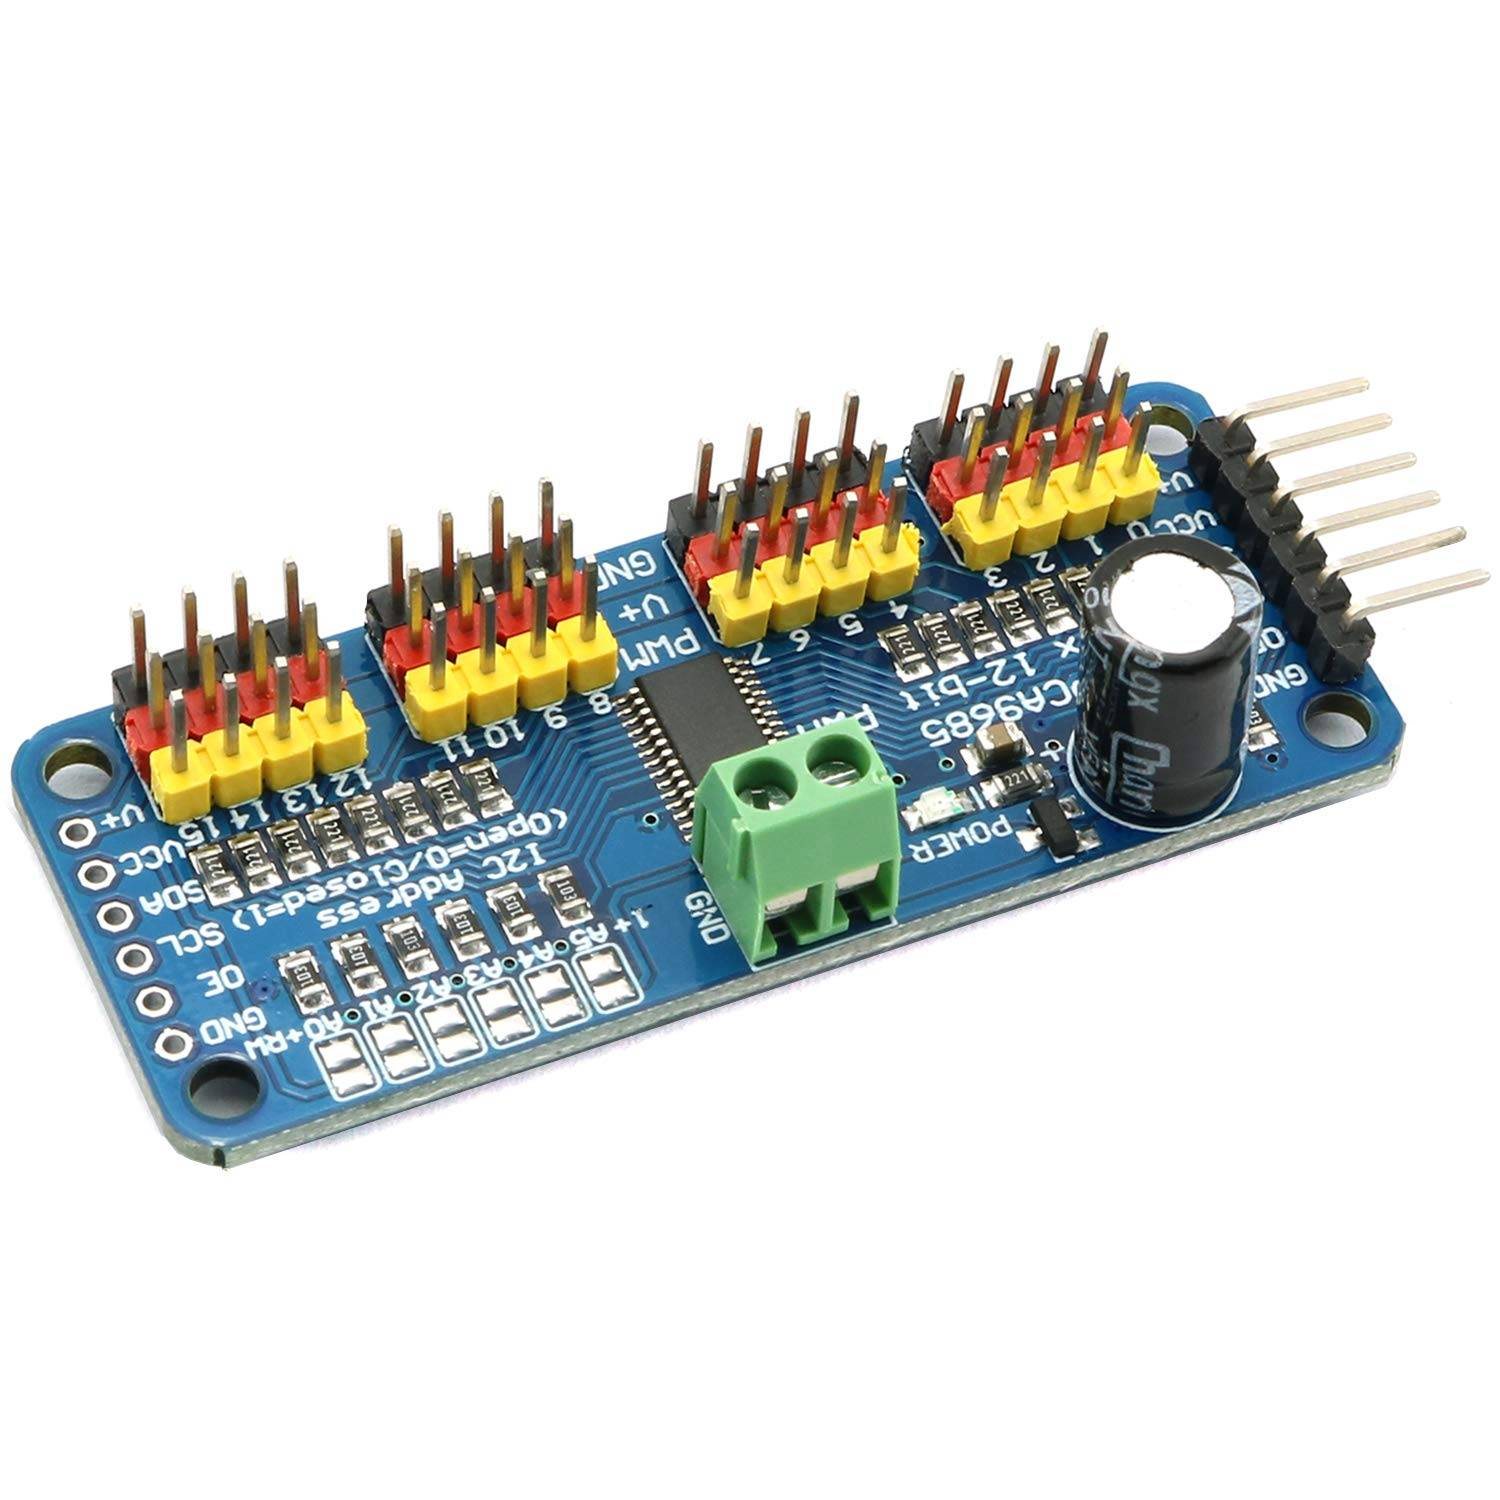
\includegraphics[width=0.5\textwidth]{pca9685}
		\caption{PCA 9685}
		\label{pca9685}
	\end{center}
\end{figure}

\subsection{Выбор инерционного датчика}\label{C4_4_3}

В ходе разработки прототипа возникла проблема с регулированием управления. Главной причиной послужило какое-либо отсутствие обратной связи у сервоприводов, о чем уже упоминалось в разделе \ref{C4_4_1}. Были предложены несколько решений данной проблемы:
\begin{enumerate}
	\item Модификация каждой платы управления сервоприводом;
	\item Подключение гироскопа акселерометра к каждому сервоприводу;
	\item Установка гироскопа акселерометра на корпусе робота.
\end{enumerate}
Первый вариант заключается в демонтаже каждого привода и прямого подключения в выходной сигнал управляющий платы.\newline 
Преимущества:
\begin{itemize}
 	\item Получение реальных углов поворота, которые принимают валы двигателей.
 	\item Нет необходимости корректировать уравнения кинематики.
 	\item Нет необходимости дополнительных вычислений, достаточно учитывать ошибку между реальным и идеальным значением на каждом шаге.
\end{itemize}
Недостатки:
\begin{itemize}
	\item Восемь аналоговых подключений.
	\item OrangePi не поддерживает аналоговые порты.
	\item Требуются дополнительные преобразовательные модули.
	\item Необходимо фильтровать данные.
\end{itemize}
Вывод:
Данное решение, не смотря на его простоту, не является подходящим, так как нет возможности его корректной реализации.
\newline


Второй метод представляет из себя снятие отклонения углов напрямую, преобразуя снятые данные с гироскопа акселерометра. Далее учитывать полученную ошибку на каждом шаге.
\newline
Преимущества:
 \begin{itemize}
 	\item Получение реальных углов поворота, которые принимают голень и бедро робота.
 	\item Нет необходимости корректировать уравнения кинематики.
 	\item Нет необходимости лишних вычислений, достаточно учитывать ошибку между реальным и идеальным значением на каждом шаге.
 	\item Получаемые данные цифровые. Это позволяет их легко обрабатывать.
 \end{itemize}
Недостатки:
\begin{itemize}
\item Гироскоп акселерометр имеет свойство накапливать ошибку. В данном случае их 8 штук, как следствие, низкая точность.
\item Восемь цифровых подключений.
\item Сложность калибровки каждого датчика отдельно.
\item Требуется дополнительный модуль "сплиттер" для подключения более двух гироскопов акселерометров.
\item Необходимо фильтровать данные.
\end{itemize}
Вывод:
Данное решение не является подходящим, так как необходимы дополнительные модули для работы с гироскопами акселерометрами в количестве более двух штук. Также существенной сложностью является калибровка большого количества датчиков и поддержание необходимой точности вычислений.
\newline


Третий метод заключается в креплении гироскопа акселерометра на корпусе робота и последующего регулировании его отклонения в плоскостях тангажа и крена, тем самым соблюдая условие комфортабельности походки, то есть реализация поступательного, равномерного и прямолинейного движения корпуса.
\newline
Преимущества:
\begin{itemize}
	\item Подключение всего одного датчика.
	\item Малые затраты на реализацию.
	\item Компенсация отклонений корпуса в плоскостях тангажа и рысканья.
	\item Получаемые данные цифровые. Это позволяет их легко обрабатывать.
\end{itemize}
Недостатки:
\begin{itemize}
	\item Необходимо корректировать уравнения кинематики.
	\item Необходимо фильтровать данные
	\item Получаемые данные цифровые. Это позволяет их легко обрабатывать.
\end{itemize}

В настоящей работе выбран третий вариант, реализация которого подробна описана в разделе \ref{C5_3}.
\subsection{Выбор источника питания}\label{C4_4_4}
Источник питания необходимо выбирать опираясь на определенные критерии. Опишем их в порядке значимости:
\begin{itemize}
	\item Высокая токоотдача для нормальной работы сервоприводов.
	\item Большая емкость для продолжительной работы.
	\item Малый вес, чтобы не увеличивать нагрузку на двигатели.
	\item Быстрая зарядка.
\end{itemize}

Таким свойствам удовлетворяет большинство Li-Po аккумуляторов, в настоящей работе была выбрана модель Spard Li-Po 3200mAh (рисунок \ref{lipo}).
\begin{figure}[h!]
	\begin{center}
		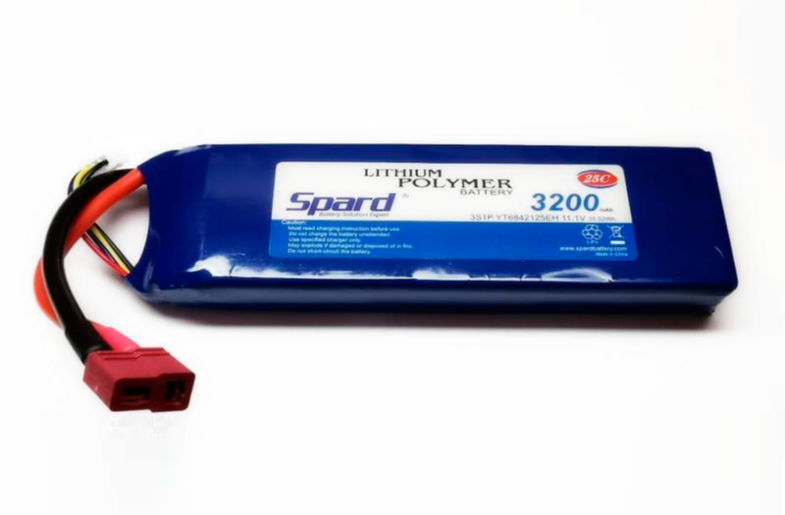
\includegraphics[width=0.5\textwidth]{lipo}
		\caption{Li-Po аккумулятор емкостью 3200 мАч}
		\label{lipo}
	\end{center}
\end{figure}


Этот тип аккумулятора получил широкое распространение благодаря своим высоким характеристикам производительности и компактности. Тип аккумуляторов Li-Po может хранить больше энергии, чем другие типы компактных источников питания, это означает, что он может работать дольше на одном заряде, что делает его идеальным для устройств, которые требуют высокой производительности и долгого времени работы. Однако, как и все, Li-Po аккумуляторы имеют некоторые недостатки. В частности, он может быть более чувствителен к перезарядке, чем другие типы аккумуляторов.Также при возможном коротком замыкании, подключенные элементы имеют высокий шанс на полный выход из строя из-за высокого порога токоотдачи. 

\textbf{Результаты проектирования и сборки} 

Финальный итог сборки робота по описанным выше твердотельным чертежам c перечисленными комплектующими представлен на  рисунках \ref{side}, \ref{back}, \ref{top}.

\begin{figure}[h!]
	\begin{center}
		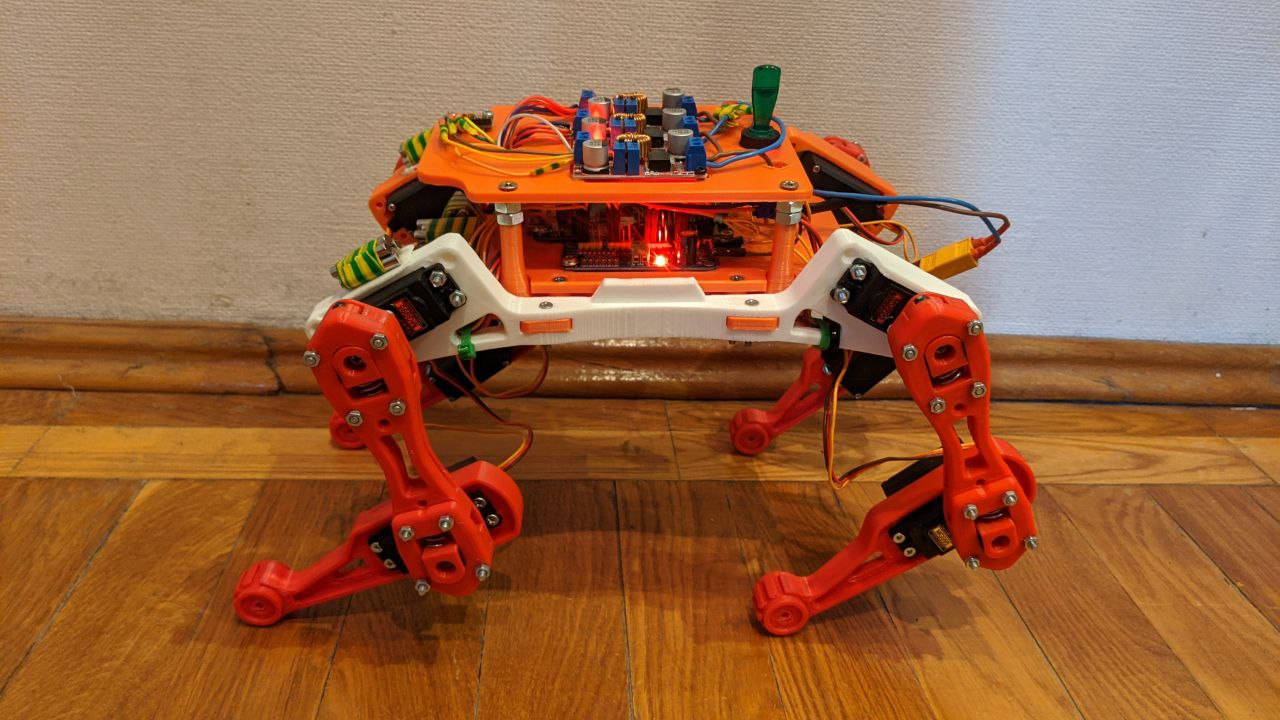
\includegraphics[width=0.9\textwidth]{side}
		\caption{Собранный прототип робота - вид сбоку}
		\label{side}
	\end{center}
\end{figure}
\newpage
\begin{figure}[h!]
	\begin{center}
		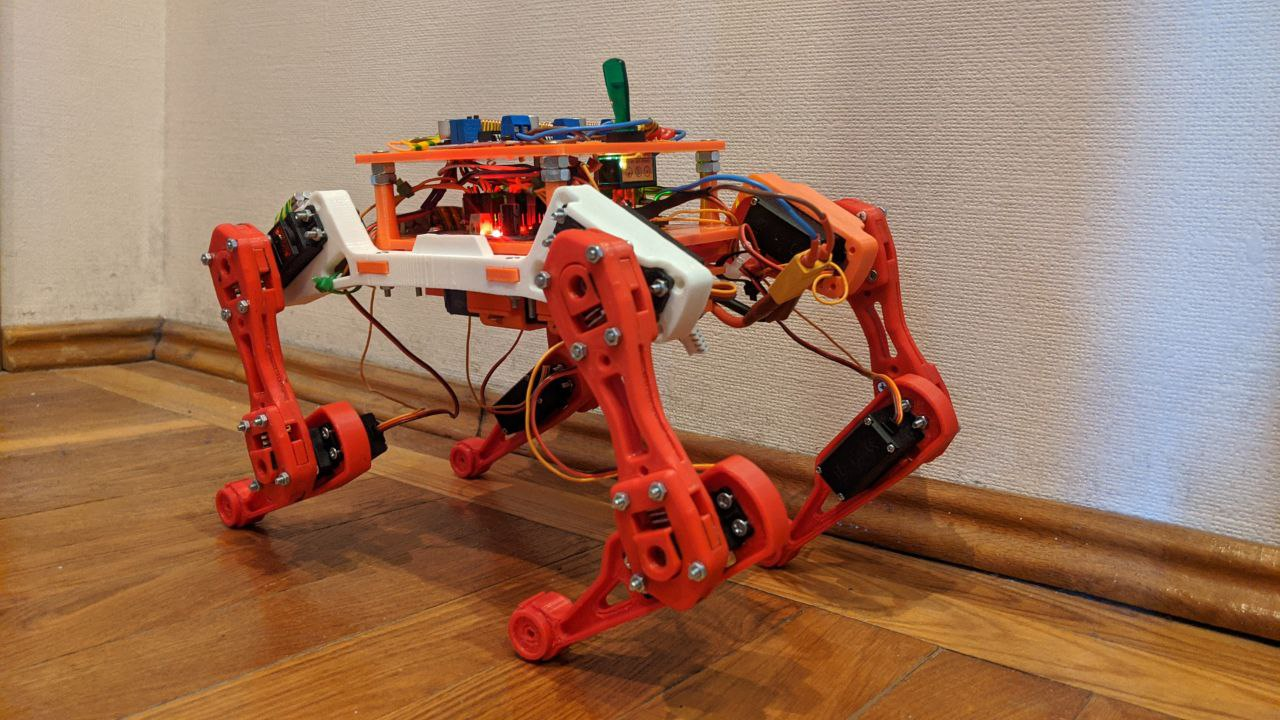
\includegraphics[width=0.9\textwidth]{back}
		\caption{Собранный прототип робота - вид сзади}
		\label{back}
	\end{center}
\end{figure}

\begin{figure}[h!]
	\begin{center}
		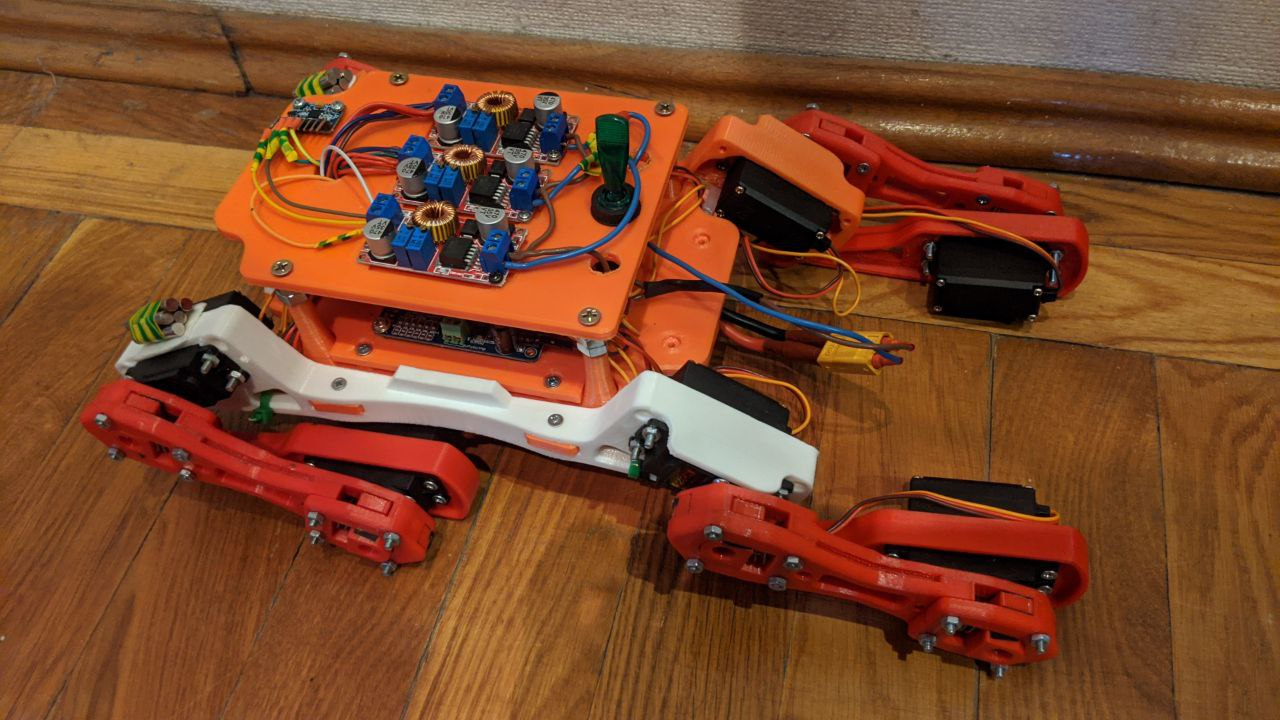
\includegraphics[width=0.9\textwidth]{top}
		\caption{Собранный прототип робота - вид сверху}
		\label{top}
	\end{center}
\end{figure}